\chapter{Caso de estudio}
\label{chp:CS}
% ---- problemas del movil
% https://www.unforgettable.org/blog/dementia-calling-phones-for-people-with-dementia/

Para este proyecto la selección de un caso de estudio que permita validar el problema de investigación planteado en el capítulo \ref{sec:Problema} es de vital importancia. Primero se realiza la búsqueda de artículos científicos que relacionan las áreas de comunicación aumentativa y alternativa (CAA), terapia ocupacional, turismo, música, tráfico y educación con los Sistemas Sensibles al Contexto, temáticas como biología/control de plagas, nutrición y noticias fueron descartadas dado que hay pocos trabajos disponibles en el estado del arte o los trabajos se orientan demasiado a la temática de los Sistemas de Recomendación Sensibles al contexto. El análisis permitió seleccionar el problema de los adultos mayores con Alzheimer como el caso de estudio, en la sección \ref{sec:CS_Comparacion} se presenta detalladamente el proceso desarrollado.\\

En la sección \ref{sec:CS_PersonasyAlz} se muestran las características de las personas con Alzheimer, luego el apartado \ref{sec:CS_Aplicaciones} se habla de los desarrollos comerciales y los trabajos de investigación relacionados, en la sección \ref{sec:Escenarios_estudio} se proponen tres casos de estudio y se desarrollan teniendo en cuenta la arquitectura presentada en el capítulo \ref{chp:Propuesta}.


cuales son los datos de contexto que incluye (clases o entidades que representa usuario, carretera, enfermedad), cómo se adquieren (dispositivos), Cuales son las entidades que me permiten representar las situaciones de mi negocio?
Me parece bueno usar algo como lo que hace \cite{Chang2017}



\section{Áreas de Aplicación para el Caso de Estudio}
\label{sec:CS_Comparacion}

Para la identificación del área de aplicación se realiza una búsqueda de los artículos indexados en Scopus, la tabla \ref{tbl:Comp_Area} presenta un resumen de los componentes encontrados en esta exploración y a continuación se presentan brevemente las características de cada área.\\



\begin{figure}[ht]
\centering%
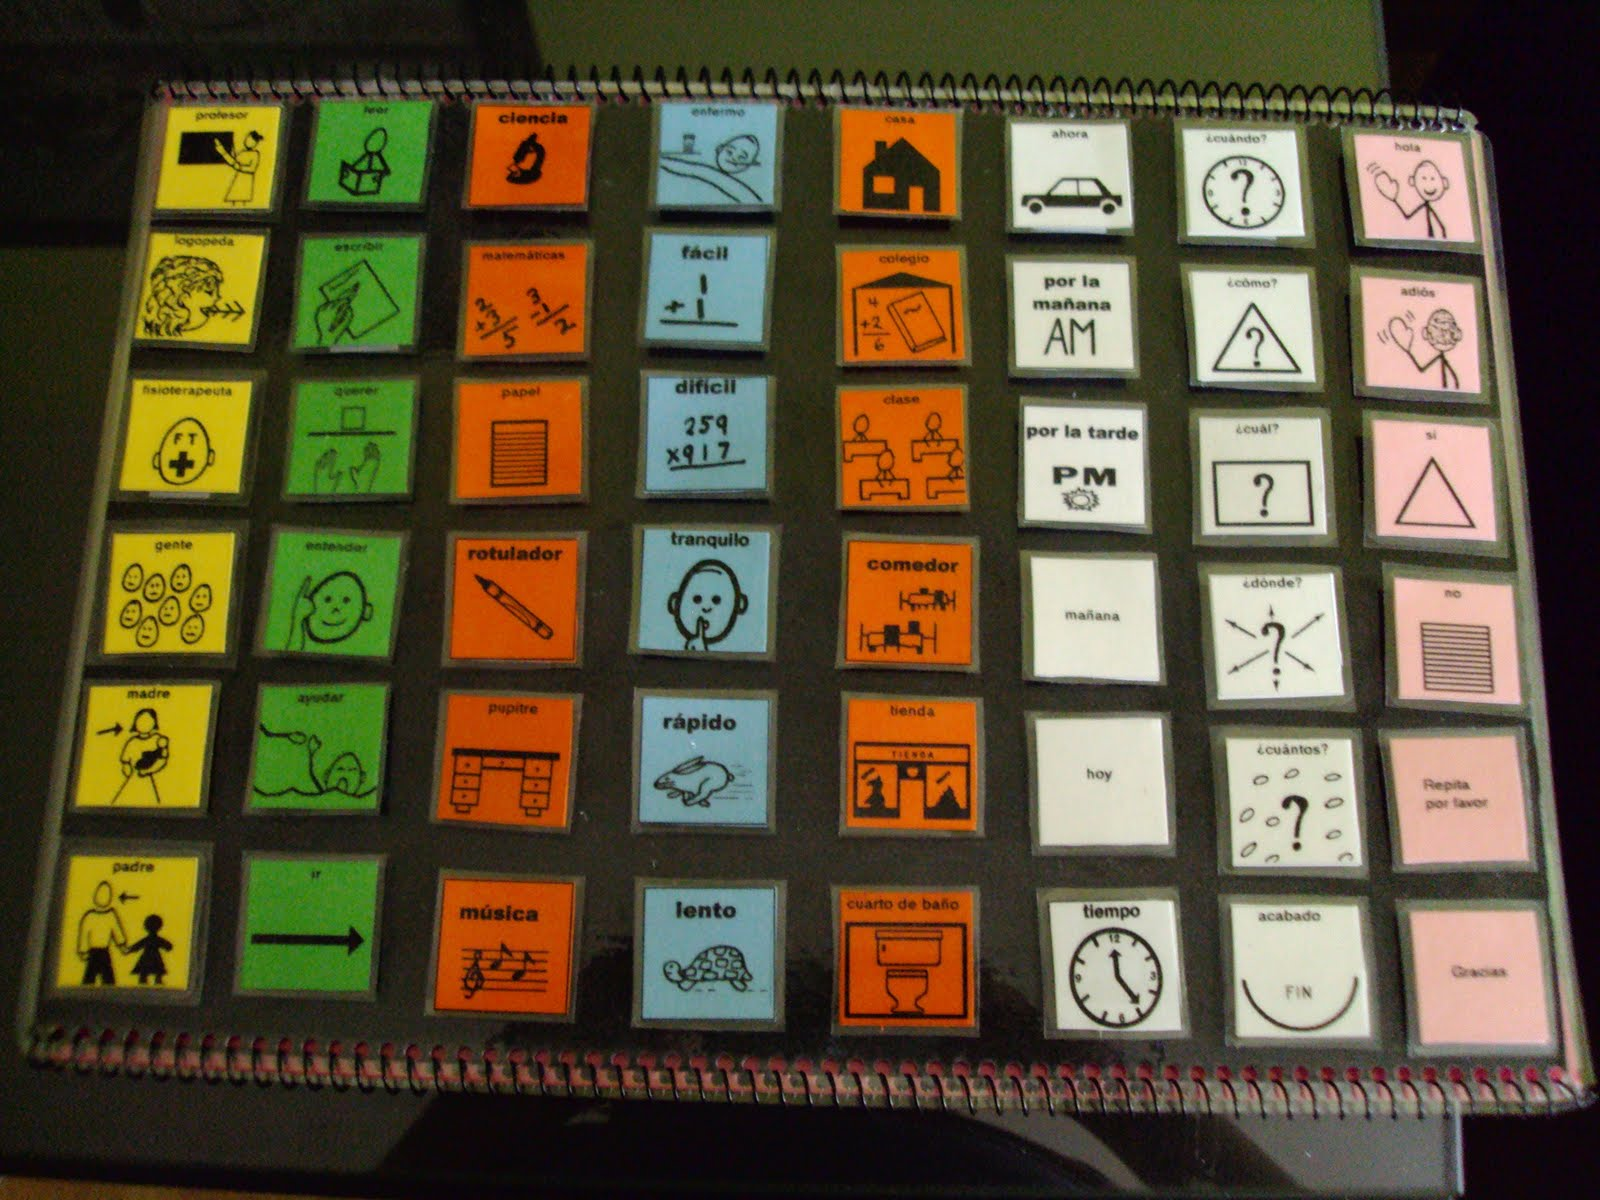
\includegraphics[width=.5\textwidth]{Cap4/tablero_convencional}%
\caption{Diagrama del Razonamiento del sistema.} \label{fig:CAA}
\end{figure}


\textbf{\textit{Comunicación Aumentativa y Alternativa (CAA)}} Los Sistemas CAA buscan formas alternativas de comunicación al lenguaje oral y escrito por medio del uso de tablas de comunicación que pueden ser digitales o análogas. La mayoría de las propuestas en esta área buscan que el usuario pueda generar frases de acuerdo al contexto que están viviendo en el momento logrando que el usuario vea solo contenidos pertinentes y que el tiempo de producción de frases disminuya. Dado que este tipo de sistemas presentan imágenes y textos, ver figura \ref{fig:CAA} estos son los contenidos multimedia que normalmente se emplean, mientras que datos provenientes de sensores como la localización, información del sistema como fecha y hora, e información del usuario como sus preferencias; son las variables contextuales de preferencia.
Resalta en esta área que al parecer no se presenta una forma de representación de conocimiento compleja, en muchos de los trabajos se realizan vínculos por medio de bases de datos de forma jerárquica por esta razón las fuentes de información son propias.\\

\textbf{\textit{Terapia Ocupacional}} En el área de terapia ocupacional se encuentran proyectos que tienen como objetivo hacer seguimiento de las actividades que desarrollan pacientes con enfermedades físicas o mentales, con este seguimiento es posible saber si un paciente ha tomado sus medicamentos, si ha desarrollado las actividades físicas recomendadas, o si se encuentra en situación de peligro. Las interfaces gráficas de estos sistemas están compuestas por imágenes, textos y vídeos que le indican al usuario las acciones que debe realizar, los usuarios normalmente no generan contenidos pero los datos que se obtienen de sensores y la información del usuario (progreso de la enfermedad etc.) son fuente principal de información para la toma de decisiones. En las propuestas encontradas no se utilizan formas de anotación de información ni se usan métodos de representación del conocimiento.\\

\textbf{\textit{Turismo}} Los sistemas sensibles al contexto en el área de turismo se caracterizan por ofrecer lugares de interés para el usuario de acuerdo a sus gustos,  \\

\textbf{\textit{Música}}
\\

\textbf{\textit{Tráfico}}
\\

\textbf{\textit{Educación}}
\\

Por lo anterior se decide combinar las áreas de ..... obteniendo .....\\

En la sección \ref{subsubsec:CS_Apli_SSC} se presenta a detalle cómo la respuesta al problema de investigación presentado en la sección \ref{sec:Problema} puede aportar al desarrollo de sistemas que faciliten la vida de las personas con Alzheimer.


 \begin{landscape}
    \thispagestyle{empty}
    \noindent
\begin{table}[h!]
\centering
\caption{Áreas de aplicación de los Sistemas Sensibles al Contexto}
\label{tbl:Comp_Area}
\begin{tabularx}{\linewidth}
{lllllll}
\hline
\multicolumn{1}{c}{\multirow{2}{*}{\textbf{Áreas}}} & \multicolumn{6}{c}{Factores}                                                                                                                                                                                                                                                   \\ \cline{2-7} 
\multicolumn{1}{c}{}                                & Aporte & \multicolumn{1}{c}{Conocimiento} & Contenidos Multimedia & \multicolumn{1}{c}{Datos de contexto} & \multicolumn{1}{c}{\begin{tabular}[c]{@{}c@{}}Formas de anotación y \\ representación del conocimiento\end{tabular}} & \multicolumn{1}{c}{Disponibilidad de datos} \\ \hline
\multicolumn{1}{c}{CAA}                             &        &                                  &                       &                                       &                                                                                                                      &                                             \\ \hline
\multicolumn{1}{c}{Terapia Ocupacional}             &        &                                  &                       &                                       &                                                                                                                      &                                             \\ \hline
Turismo                                             &        &                                  &                       &                                       &                                                                                                                      &                                             \\ \hline
Música                                              &        &                                  &                       &                                       &                                                                                                                      &                                             \\ \hline
Tráfico                                             &        &                                  &                       &                                       &                                                                                                                      &                                             \\ \hline
Educación                                           &        &                                  &                       &                                       &                                                                                                                      &                                             \\ \hline

\end{tabularx}
    \end{table}
  \end{landscape}


\section{Personas mayores y Alzheimer}
\label{sec:CS_PersonasyAlz}

En Colombia se considera Adulto Mayor a la persona que alcanza los 60 años de edad, en el año 2013 esta población representó el 10\% del total de la población del país (4.962.491) y se estima que en el 2020 hayan 49 adultos mayores por cada 100 menores de 15 años. Esta cifra indica la necesidad de desarrollar sistemas que permitan lidiar con las complicaciones que representa la transición a la vejez \cite{ministeriodesalud2013}. Los adultos mayores experimentan cambios físicos y mentales que cambian sus rutinas y los hacen dependientes de familiares y cuidadores, la demencia es un síndrome mental que afecta la memoria, la programación de actividades y los movimientos de la persona según el grado y tipo de afectación \cite{Fargo2014}.

El Alzheimer es el tipo de demencia más común, sus etapas finales se caracterizan porque la persona pierde habilidades como caminar o tragar por lo cuál se le considera una enfermedad fatal. Diferentes factores llevan al desarrollo de la enfermedad \textbf{\textit{(i)}} edad mayor a 65 años, \textbf{\textit{(ii)}} familiares en primer grado con la enfermedad, \textbf{\textit{(iii)}} afectaciones cardiovasculares, \textbf{\textit{(iv)}} falta de actividades sociales y cognitivas, y finalmente \textbf{\textit{(v)}} heridas en el cerebro. En la actualidad el Alzheimer no tiene cura por lo tanto los tratamientos se concentran en disminuir el progreso de la enfermedad \cite{Fargo2014}.

Monteagudo \cite{monteagudo2014capacidades} identifica diferentes áreas de acción de las TIC en la enfermedad, dentro de estas áreas sobresalen \textbf{\textit{(i) el tratamiento}} que busca prevenir, parar o revertir la enfermedad por medio de la estimulación cognitiva, la actividad física, de la voz y el lenguaje,y el procesamiento de las señales producidas por sensores. Y \textbf{\textit{(ii) la mejora de calidad de vida de los pacientes y cuidadores}} en dónde la mayoría de implementaciones se concentran en la mejora de la comunicación social de los pacientes pero se ha empezado a trabajar en estrategias que le den independencia al paciente para la realización de actividades del diario vivir.

Como se nombra en la sección \ref{sec:Escenarios_estudio} este proyecto tiene en cuenta en sus escenarios a personas con un nivel leve de Alzheimer, según la \textit{Fundación de Azheimer de America}\footnote{https://alzfdn.org/caregiving-resources/about-alzheimers-disease-and-dementia} este nivel se caracteriza por \textbf{\textit{(i)}} Perdida de memoria, \textbf{\textit{(ii)}} confusión en tiempo y espacio, \textbf{\textit{(iii)}} dificultad al desarrollar tareas sencillas como cepillarse los dientes, \textbf{\textit{(iv)}} problemas para encontrar palabras y \textbf{\textit{(v)}} cambios de ánimo y personalidad. 


\section{Aplicaciones existentes para Alzheimer}
\label{sec:CS_Aplicaciones}

\subsubsection{Aplicaciones Comerciales}

En la web se puede encontrar bastante información acerca de lo que necesitan los pacientes con Alzheimer para tener una buena calidad de vida y disminuir el progreso de la enfermedad. Por ejemplo Carezone\footnote{www.carezone.com} permite hacer un listado de las medicinas que debe tomar un paciente, hacer un horario para la toma de los medicamentos e incluir a los contactos más importantes en casos de emergencia. Symple Symptom Tracker \footnote{www.sympleapp.com} permite a los usuarios registrar su ánimo en diferentes aspectos como ansiedad, dolor y sueño; adicionalmente funciona como un diario que registra las horas de sueño, ritmos cardiacos entre otros. De otro lado Elevate \footnote{www.elevateapp.com} es una aplicación para ejercitar el cerebro a partir de diferentes juegos entre los que se encuentra la escritura, comprensión de lectura, habilidades matemáticas, entre otros. Finalmente en el mercado se pueden encontrar aplicaciones que usan tecnologías GPS para mantener al cuidador informado de la ubicación de las personas con Alzheimer e incluso definir zonas de peligro en cuyo caso el dispositivo dará alertas a las personas registradas como el caso de Tweri \footnote{www.tweri.com}

\subsubsection{Sistemas Sensibles al Contexto y Alzheimer}
\label{subsubsec:CS_Apli_SSC}
En bases de datos como Scopus son pocos los trabajos que relacionan directamente los SSC y el Alzhaimer, Taub et al.\cite{Taub2011TheEscort} propone un sistema que monitorea a la persona y envía alertas cuando esta se encuentra en un lugar peligroso, adicionalmente es posible saber la ubicación de la persona dentro de un edificio y enviar alertas si se ingresa o se ha estado en un lugar por mucho tiempo. % mejorar 
Un trabajo más reciente elaborado por Pulido \cite{PulidoHerrera2017} presenta una recopilación de trabajos que se centran en usar tecnologías de localización para ayudar a las personas mayores cuando estas se extravían, en el área de los SSC se puede concluir que las propuestas buscan combinar la información de la localización del usuario con la del ambiente que esta recorriendo (clima, seguridad, etc) y también buscan aplicar estrategias de inteligencia artificial para aprender la rutina de las personas con Alzheimer e identificar si estas se encuentran en peligro.

Kanai \cite{Kanai2012} crea un hogar grupal sensible al ambiente para adultos mayores con demencia por medio del uso de sensores de movimiento, RFID, entre otros. El sistema emplea redes bayesianas que permiten reconocer si ha ocurrido o va a ocurrir un accidente dentro del hogar, gracias a esto los cuidadores pueden actuar rápidamente modificando el entorno de las personas con la enfermedad.\cite{Zolfaghari2016} en años más recientes Zolfaghari propone el uso de casas inteligentes y la inteligencia del ambiente para percibir las variables de los usuarios y el entorno. Las señales que son producidas por los sensores son analizadas y por medio del uso de ontologías se identifica la actividad que se está desarrollado. % mejorar, leer mas porque tiene mucha información de utilidad.
Navarro et al. \cite{Navarro2012, Navarro2016} presenta un Sistema de Memoria de Ambiente que aumenta la información de personas, lugares y cosas para ayudar a los adultos mayores con Alzheimer. El sistema usa ontologías para modelar la información del paciente y el sistema cambia su comportamiento de acuerdo a eventos relacionados con la enfermedad, adicionalmente información relevante se muestra al usuario por medio de una pantalla táctil y el cuidador puede modificar la información del sistema por medio de un celular inteligente.%leer el de 2016 (complementa la información)
Griol y Callejas \cite{Griol2016} presentan un sistema de agentes de conversación multimodal sensible al contexto para aplicaciones Android que se adaptan a las necesidades del usuario, el principal objetivo de esta propuesta es preservar las habilidades cognitivas y mejorar las relaciones con el entorno de las personas con Alzheimer. Cabe resaltar que los agentes de conversación multimodal se refieren al uso de diferentes modos de interacción para comunicar información a los dispositivos, estos modos pueden ser táctil, voz, reconocimiento de imágenes, o una combinación de ellas. %ESTE TIENE QUE SER UNA REFERENCIA
\\

\textit{\textbf{DEBEMOS REVVISAR ESTO}}
Aunque algunos trabajos buscan facilitar las actividades que realizan los cuidadores de personas con Alzheimer por medio de la obtención del contexto a partir de la localización y algunos sensores en entornos inteligentes, y otras propuestas buscan mantener la memoria de los pacientes, existe una brecha en la aplicación de los sistemas sensibles al contexto para el desarrollo de aplicaciones que aumenten la calidad de vida y la independencia de los usuarios con este tipo de demencia. Teniendo en cuenta que la \textbf{\textit{COMPUTACIÓN UBICUA}} se hace realidad cada día es posible usar no solo los contenidos que puede crear una persona durante el desarrollo de sus rutinas sino los datos que generan los dispositivos de forma automática y continua.
La combinación de los datos de los sensores, la multimedia que produce un usuario y el contexto en el cual se producen estos contenidos puede ser de grán utilidad para el desarrollo de la vida personal de un usuario que olvida los componentes más importantes de su vida.



Ya que los trabajos que se encuentran en el estado del arte exploran el uso de sensores para identificar el contexto de un usuario y modificar las acciones de los dispositivos, la aplicación de los escenarios permiten observar cómo la adición de contenido multimedia puede apoyar en la definición del contexto de una persona con Alzhaimer.

\section{Escenarios de estudio}
\label{sec:Escenarios_estudio}

Para la selección y desarrollo de los escenarios de estudio se tiene en cuenta el trabajo de Monteagudo \cite{monteagudo2014capacidades}, el proponen dos escenarios en dónde se aplican las tecnologías de la información de acuerdo al nivel de Alzheimer que tiene una persona. El primer caso refleja el mundo de los pacientes con Alzheimer leve, donde sobresale la necesidad de educar a las personas a envejecer con su enfermedad y a generar herramientas que les permita una vida independiente de forma segura y social por lo tanto es pertinente para el desarrollo de esta tesis.

Dada la cercanía de los adultos mayores a la población objetivo ...
%HABLAR DE LA POBLACIÓN Y CÓMO SE VA A EVALUAR
\\

\textbf{\textit{Escenario 1:}} Ivan tiene diabetes y el poco cuidado que le ha dado a su enfermedad ha desencadenado un nivel leve de Alzheimer que pasa progresiva y rápidamente a un nivel intermedio. Al salir de su casa Ivan le dice a su hija que irá a dar un paseo por la ciudad ella le pregunta a donde quiere ir pero Ivan no le responde, desde hace algunas semanas le molesta que le pregunten a donde va pues siente que lo controlan por esta razón también deja el teléfono celular en su casa.
Después de caminar un par de kilómetros Ivan tropieza con un objeto en la calle y cae al suelo, al reaccionar se da cuenta que no sabe dónde se encuentra ni qué actividad estaba realizando, las personas que caminaban por la calle lo socorren pero no saben que pueden hacer para ayudar a Ivan.\\

\textbf{\textit{Escenario 2:}} Es de noche y Luís se encuentra hablando con su hija en su casa, ella le pregunta por las actividades que realizo en el día y las que realizó el día anterior pues no pudo ir a visitarlo. Luís se da cuenta que tiene recuerdos vagos de lo que hizo, sabe que los dos días tuvo todas las comidas y que en las tardes tomó la siesta pero no sabe exactamente en dónde estuvo ni con quién.
Mariana, la hija de luís, le recomienda que lleve un registro de lo que hace en una libreta y que tome con su celular vídeos y fotos para que sea más fácil recordar las actividades realizadas. Al otro día Luís compra una libreta y empieza a registrar las actividades que desarrolla en el día, ahora puede decirle fácilmente a sus familiares que hizo en días pasados, aunque escribe que estuvo en un centro comercial pero no recuerda con exactitud en cual.\\

\textbf{\textit{Escenario puntual:}} El usuario observa una fotografía tomada hace dos semanas en horas de la noche, el usuario se encuentra rodeado de varias personas, a algunas las recuerda y a otras no. Tampoco recuerda cuál fue el clima ese día pero si que recuerda el lugar en el que se encontraba.\\
\begin{itemize}
\item \textbf{variables contextuales:} Día y Hora, Localización, Estado del tiempo y Social.
\item \textbf{Multimedia:} Imágenes.
\item \textbf{Sensores:} GPS, fuente externa con datos del clima de un lugar.
\end{itemize}



%IMPORT DE LA TABLA
\begin{table}[ht!]
\centering
\caption{Atributos de los escenarios de estudio}
\label{tbl:Esce_Analisis}

\begin{tabularx}{\textwidth}{@{}lllll@{}}
\toprule
\multicolumn{1}{c}{\textbf{Escenarios}} & \multicolumn{1}{c}{\textbf{\begin{tabular}[c]{@{}c@{}}Interfaz /\\ Interacción\end{tabular}}} & \multicolumn{1}{c}{\textbf{Opciones}}                                                                                                                                                                        & \multicolumn{1}{c}{\textbf{Dispositivos}}                                       & \multicolumn{1}{c}{\textbf{Sensores}}                                                               \\ \midrule
Escenario 1                             & \begin{tabular}[c]{@{}l@{}}Mapa\\ Mensajes alerta\\ Producción de voz\end{tabular}            & \begin{tabular}[c]{@{}l@{}}Ver ubicación del usuario\\ Recibir alertas de eventos identificados\\ Comunicarse con cuidador\\ Identificación de actividades desarrolladas\end{tabular}                        & \begin{tabular}[c]{@{}l@{}}Celular inteligente\\ Reloj inteligente\end{tabular} & \begin{tabular}[c]{@{}l@{}}GPS\\ Acelerometro\\ Pulsometro\\ Cámara\end{tabular}                    \\
Escenario 2                             & Historia del usuario                                                                          & \begin{tabular}[c]{@{}l@{}}Captura Multimedia\\ Asistencia para la construcción de historias\\ Compartir contenidos\\ Reconocimiento y almacenamiento de actividades\\ Conversión audio a texto\end{tabular} & \begin{tabular}[c]{@{}l@{}}Celular inteligente\\ Wereable devices\end{tabular}  & \begin{tabular}[c]{@{}l@{}}GPS\\ Acelerometro\\ Pulsometro\\ Cámara\\ Micrófono\\ ....\end{tabular} \\ \bottomrule


\end{tabularx}

\end{table}


Cada uno de los escenarios fue analizado buscando las posibilidades que debía ofrecer en tres áreas interfaz gráfica, opciones para el usuario, dispositivos y sensores; una tabla con el resumen del análisis se puede encontrar en la tabla \ref{tbl:Esce_Analisis}. Finalmente se enfrentan las opciones y sensores identificados contra la arquitectura formulada en el capítulo \ref{sec:Prop_Arquitectura}.

Teniendo en cuenta el desarrollo de los escenarios es posible que los usuarios deban tener un dispositivo que envía información en todo momento, como el sensor GPS o una cámara que facilite el reconocimiento de rostros.

\subsection{Riesgos}\cite{Fargo2014}

\section{Información contextual y conjunto de datos}

\textbf{dEBERÍA RESPALDARLO CON ALGÚN PROFESIONAL EN EL ÁREA}
Localización
Hora y Día
Clima
Sociedad
Emoción
Dispositivos

Tipo de contexto | Razón de la inclusión


(multimedia)

\section{Conjunto de datos}
\label{sec:Prop_Conj_Datos}

Como se indica en la sección \ref{chp:Marco_Teorico} \textbf{PONER CONTEXT AWARENESS} los sensores son la fuente principal de datos para los Sistemas Sensibles al Contexto, en el caso de la adquisición de contexto en entornos cerrados los entornos inteligentes permiten estudiar el reconocimiento de actividades y la asistencia y monitoreo a pacientes y a personas de la tercera edad. Alemdar et al. \cite{Alemdar2013} presenta un conjunto de datos compuesto por sensores dispuestos en diferentes lugares de dos hogares para registrar las actividades realizadas durante dos meses, en este trabajo se resalta la necesidad de identificar los sensores influyen en menor medida en la realización de actividades y también el uso adecuado de la energía en cada uno de los dispositivos para evitar la carga constante de los mismos. OTRO

Teniendo en cuenta que la creación de conjuntos de datos desde el mundo real es complicado propuestas como \cite{} proponen la creación de conjuntos de datos sintéticos. 

En la actualidad no es posible encontrar conjuntos de datos que combinen los datos de sensor con contenidos multimedia, por tal razón se decide --------

https://www.kaggle.com/

\section{Ontología del dominio}
\label{sec:CS_Ont_Dominio}

Llenar la ontología en lugares con códigos de GeoNames :v  (http://www.geonames.org/export/codes.html)

También puedo mirar este http://mklab.iti.gr/project/prophet-ontology-populator

\section{Tranformación de datos}

\todo{Ver este artículo, está en mendeley}
GPS Trajectory Linked Open Data based on Open POI Information-Through an Experiment in ISWC2016- 2 Experiments for collecting GPS trajectory data in ISWC2016

Linked data me puede servir para tener el nombre del lugar en el que está la persona y si es el caso ponerlo como individual en la ontología, así el no tiene que poner la información manualmente!